\documentclass[12pt, oneside]{article}
\usepackage{amssymb,amsmath}
\usepackage{textpos}
\usepackage{systeme}
\usepackage{bm}
\usepackage{qtree}
\usepackage{listings}
\usepackage{graphicx} 
\usepackage[outdir=./]{epstopdf}
\usepackage{mathtools,xparse}
\usepackage{multirow}

\usepackage{setspace}
\usepackage[margin=1in, top=20mm, bottom=20mm]{geometry}
\usepackage[dvipsnames]{xcolor}
\usepackage{titlesec}
\definecolor{teagreen}{rgb}{0.82, 0.94, 0.75}
\usepackage{hyperref}
\newcommand{\irref}[2]{\hyperref[#2]{#1~\ref{#2}}}

\usepackage{subcaption}
\usepackage{caption}


\begin{document}
\doublespacing


\begin{titlepage}
    \begin{center}
        \vspace*{1cm}
 
        \Huge
        \textbf{Sluice: A Network-Wide Model for Data Plane Programming}
 
        \vspace{0.5cm}
        \Large
 
        \vspace{1.5cm}
 	by\\
        \textbf{Vikas Natesh}\\
 	Advisor : Dr. Anirudh Sivaraman    \_\_\_\_\_\_\_\_\_\_\_\_\_\_\_\_\_\_\_\_\_\_\_\_\_\_\_\_\_\\
	Examiner : Dr. Aurojit Panda \_\_\_\_\_\_\_\_\_\_\_\_\_\_\_\_\_\_\_\_\_\_\_\_\_\_\_\_\_
        \vfill
 
        \large
        A thesis submitted in partial fulfillment \\
        of the requirements for the degree of\\
		Master of Science
 
        \vspace{0.8cm}
  
        Department of Computer Science\\
        Courant Institute of Mathematical Sciences\\
        New York University\\
        May 2019
 
    \end{center}
\end{titlepage}

\begin{abstract}
Networking devices have traditionally been thought of as fixed-function devices that perform the single task of packet switching very well. However, in recent years, researchers have developed network devices that can be explicitly programmed to perform complex packet processing tasks. These devices, which include routers, network interface cards (NICs), and middleboxes can support applications such as load balancing, heavy-hitter detection, and improved packet scheduling. While greater control over each device allows for better visibility into the network, it is still difficult to program the network as a whole. In the current state, network operators are required to program each individual device using a language such as P4 or Micro-C in order to express a network-wide computation. This thesis presents Sluice, a programming model that takes a high-level specification of a network program, and compiles it into runnable code that can be launched on the programmable devices of network. We describe the design and language features of Sluice and compare it side-by-side to equivalent P4 translations. Finally, we run through several demos where Sluice is used to program a virtual network of programmable switches and hosts in a Mininet emulator.
\end{abstract}

\newpage
\section*{Acknowledgements}

\newpage
\tableofcontents

\newpage
\listoffigures

\newpage
\lstlistoflistings

\newpage
\section{Introduction}
The last several years have seen the emergence of programmable network devices
including both programmable switching chips and programmable network interface
cards (NICs). Along with the rise of x86-based packet processing for
middleboxes and virtual switches, these trends point towards a future where the
entire network will be programmable. The benefits of network programmability
range from commercial use cases such as network virtualization implemented on
the programmable Open vSwitch platform to more recent research projects that
implement packet scheduling, measurement, and application offload of niche
applications on programmable switches.

While the benefits of programmability are clear, they are difficult to reap
because programming the network as a whole remains challenging. Current
programming languages target individual network devices, e.g., P4 for the
Tofino programmable switching chip and the Netronome programmable NIC. However,
at present, there is no unified programming model to express and implement
general data plane functionality at the level of an entire network, without
having to individually program each network device.

Prior work has looked at the problem of programming at the level of an entire
network. In particular, Maple~\cite{maple} was an early example of a
network-wide programming model designed for OpenFlow switches. Maple
automatically divided functionality between a stateless component running on
switches and a stateful component running on the network's controller.
SNAP~\cite{snap} is a more recent example of network-wide programming; unlike
Maple, it additionally offloads stateful functionality to switches by
leveraging stateful processing available in programmable switches.  However,
both Maple and SNAP cannot express programmable-switch functionality that
affects network performance at fine time scales, e.g., packet scheduling,
congestion control, fine-grained measurement of microbursts, and load
balancing. In other words, Maple and SNAP generate highly optimized code, but
are restricted in what they can express.

This thesis presents \textbf{Sluice}, a programming model that takes a
network-wide specification of the data plane and compiles it into runnable code
that can be launched directly on the programmable devices of a network. In
contrast to prior network-wide programming models like SNAP and Maple that were
focused on specific tasks (e.g., routing and security policies), Sluice aims to
be more general, but potentially at the cost of quality of generated code.
Sluice endows network operators with the ability to design and deploy large
network programs for various functions such as scheduling, measurement, and
application offloading.  The benefits of Sluice can be summarized as follows:\\
\quad  (1) Sluice provides the same functionality as a per-device language like P4 but makes it easier to program the data plane of an entire network by abstracting device-specific architectural details like stateful ALUs, pipelines, etc., and\\
\quad  (2) Sluice automatically reduces the amount of boilerplate code needed to write data plane functionality. For instance, the 8 line traffic matrix Sluice program (which we demonstrate later) translates into over 200 lines of P4 code. 

\begin{figure}
\centering
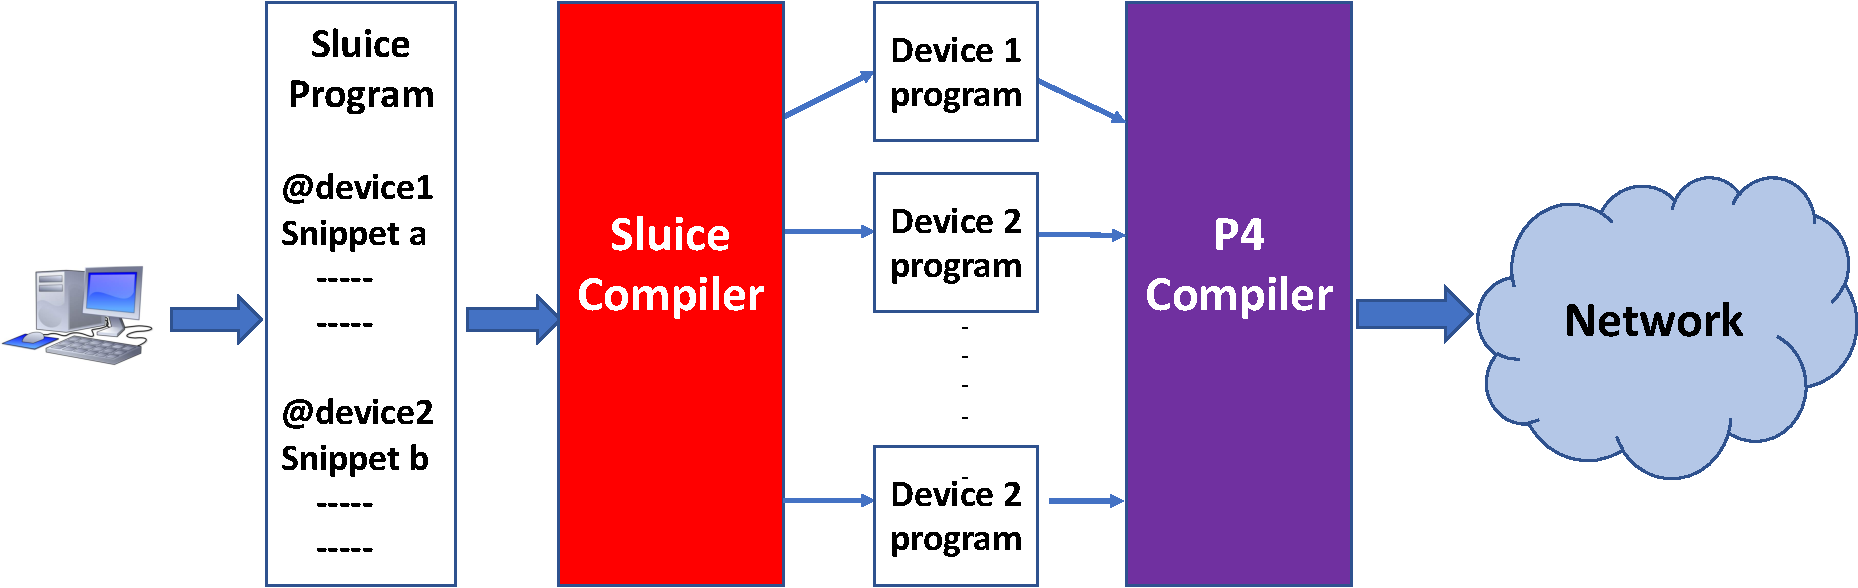
\includegraphics[width=140mm,scale=0.7]{figures/sluice_workflow.pdf}
\caption{Sluice Workflow}\label{fig1}
\end{figure}

\newpage
\section{Sluice Overview}
In the Sluice model, a network-wide program consists of high-level code
\textit{snippets} annotated by the operator to run on particular devices in a
network. The code in each snippet is to be executed on packets arriving at its
corresponding device. Snippets support a variety of operations:
read-from/write-to packets; arithmetic using packet headers, local variables, or
stateful register arrays; and control flow statements. To handle computation on
custom packet headers not supported by default (eth/ip/tcp/udp), users may
define packet header declarations similar to C structs. An optional annotation
in the declaration, the parser condition, automatically generates a header
parser for these user-defined headers. Sluice programs may also import
device-specific variables/attributes for use in code snippets. Sluice also lets
the programmer restrict snippets to operate on specific flows or IP address
ranges.

\irref{Figure}{fig1} describes the Sluice workflow. The compiler translates each snippet of
a sluice program into a device-specific program. After initial parsing, lines
of code in the snippet are decomposed into a directed acyclic graph (DAG) that
maps dependencies between variables in each snippet. This graph is then passed
to the backend of the compiler that generates the corresponding P4 program for
that device, for example bmv2 or Tofino.\footnote{Currently we only support
bmv2 but plan to support more devices.} 

If successfully compiled into P4, Sluice programs are guaranteed to run at line rate on the switch. However, the need for line rate performance precludes the ability to perform looping in Sluice such as \texttt{for} and \texttt{while}. Although looping semantics can be implemented by recirculating packets back into the ingress pipeline of the switch (to repeat some computation)~\cite{p4Spec}, this significantly reduces throughput. Nonetheless, fairly complex algorithms can still be expressed without loops. This is discussed further in the demonstrations section. 

\newpage
\section{Design and Implementation}

\begin{lstlisting}[basicstyle=\linespread{1.3}\scriptsize,  numberstyle=\tiny, backgroundcolor = \color{teagreen}, frame=tlrb]
program:
	imports packets snippets				
	| packets snippets
\end{lstlisting}

The Sluice compiler is built using the Rust system programming language, chosen for its memory safety, variable lifetime management, and high performance. This section details the language specification. The following conventions are used:

\begin{itemize}
  \item The GNU Bison grammar is used to display production rules. Boxes containing the grammar are shaded light-green.
  \item Terminal symbols are indicated in caps and constant string tokens are indicated in double quotes.
  \item A vertical bar, $|$, separates options from which exactly one must be selected.
  \item Curly braces, colons, and semicolons ending statements have been omitted for clarity.
  \item The 'Empty' keyword in the grammar indicates an empty string.
  \item Symbols marked as IDENTIFER or *\_ID represent names of files, variables, packets, snippets, packet fields, etc.
\end{itemize}


\subsection{Imports}
\begin{lstlisting}[basicstyle=\linespread{1.3}\scriptsize,  numberstyle=\tiny, backgroundcolor = \color{teagreen}, frame=tlrb]
imports:
	imports import
	| import
	;
import:
	"import device" IMPORT_ID
	;
\end{lstlisting}

The import\_id represents the name of an external file in which an operator may declare several target-specific fields. These fields can then be read and used within code snippets. For instance, the bmv2 target supports access to the enqueue depth of the virtual switches in a topology. By default, Sluice supports the P4 portable switch architecture (PSA) fields, defined in the "psa.np" file. 

\begin{lstlisting}[basicstyle=\linespread{1.3}\scriptsize, caption=PSA fields]
device psa {
  timestamp_rx : bit<48>;
  timestamp_ingress : bit<48>;
  timestamp_egress : bit<48>;
  timestamp_tx : bit<48>;
  ingress_port : bit<9>;
  egress_port : bit<9>;
  packet_length : bit<32>;
  enq_qdepth : bit<32>;
  deq_qdepth : bit<32>;
}
\end{lstlisting}



\subsection{Packets}
\begin{lstlisting}[basicstyle=\linespread{1.3}\scriptsize,  numberstyle=\tiny, backgroundcolor = \color{teagreen}, frame=tlrb]
packets:
	packets packet
	| packet
	;
packet:
	"packet" PACKET_ID packet_base packet_parser_condition packet_fields
	;
packet_base:
	"tcp" | "udp" | "ipv4" | "ethernet"
	;
packet_fields:
	packet_fields packet_field
	| packet_field
	;
packet_field:
	IDENTIFIER var_type type_qualifier
	;
packet_parser_condition:
	IDENTIFIER value
	| Empty
	;
\end{lstlisting}

Packets are declared similarly to C structs. Within a packet declaration, users can define custom packet headers which can be used for computation in code snippets. In addition, all (eth/ip/udp/tcp) header fields are supported by default. The \texttt{packet} keyword is followed by a packet\_base and an optional packet\_parser\_condition. These two attributes help Sluice automatically generate a P4 packet header parser. The packet\_base is a string of either $tcp$, $udp$, $ipv4$, or $ethernet$ and represents the header type on which to parse the packet.  Meanwhile, the parser condition defines the header field and value to match incoming packets on. Packets that do not pass the parser condition are immediately sent to the ingress pipeline. However, to restrict the operation of Sluice snippet code to only those packets that passed the condition, a P4 \texttt{if} statement is automatically generated in the ingress control block. In this way, the parser condition allows the operator to conditionally perform computation on different flows.

\begin{figure}
\caption{P4 Translation for Sluice Parser Condition}\label{pca}
\noindent\begin{minipage}{.45\textwidth}
\begin{lstlisting}[basicstyle=\linespread{1.3}\scriptsize, title={Sluice Parser Condition},frame=tlrb]{Name}
packet p: udp(srcPort:1234) {
  nhops : bit<32>;
}
\end{lstlisting}
\begin{lstlisting}[numbers=left, firstnumber=1, title={P4 Ingress Control Block}, basicstyle=\linespread{1.3}\scriptsize, frame=tlrb]
control ingress {
  if (udp.srcPort == 1234 && 
   ethernet.etherType == ETHERTYPE_IPV4 
   && ipv4.protocol == IP_PROTOCOLS_UDP){
		.
		.
		.
	*** SNIPPET P4 CODE ***
		.
		.
		.
	}
  if(valid(ipv4) and ipv4.ttl > 0) {
      apply(ipv4_lpm);
    }
\end{lstlisting}

\end{minipage}\hfill
\begin{minipage}{.45\textwidth}
\begin{lstlisting}[title={P4 Parser},frame=tlrb, basicstyle=\linespread{1.08}\scriptsize]
parser start {
    return parse_ethernet;
}
parser parse_ethernet {
    extract(ethernet);
    return select(latest.etherType) {
        ETHERTYPE_IPV4 : parse_ipv4;
        default: ingress;
    }
}
parser parse_ipv4 {
    extract(ipv4);
    return select(latest.protocol) {
        IP_PROTOCOLS_TCP : parse_tcp;
        IP_PROTOCOLS_UDP : parse_udp;
        default: ingress;
    }
}
parser parse_tcp {
    extract(tcp);
    return ingress;
}
parser parse_udp {
    extract(udp);
    return select(latest.srcPort) {
        1234 : parse_p;
        default: ingress;
    }
}
parser parse_p {
    extract(p);
        return ingress;
}
\end{lstlisting}
\end{minipage}
\end{figure}


In \irref{Figure}{pca}, the packet $p$ contains a single field $nhops$ that is used by the operator to maintain a hop count on each packet. It is parsed on the udp $srcPort$ field.  The corresponding P4 header parser and control block are also shown. In particular, the $parse\_udp$ parser shows that headers of packet $p$ (nhops in this example) are extracted only when $\texttt{srcPort}=1234$. In the ingress block, the \texttt{if} statement on lines 2-4 ensures that P4 code corresponding to Sluice snippets are only executed on packets that have $udp.srcPort = 1234$. All other packets are sent to the routing table ipv4\_lpm, provided that they have a valid ipv4 header i.e. they are simply routed and do not affect router state.



\subsection{Snippets}
\begin{lstlisting}[basicstyle=\linespread{1.3}\scriptsize,  numberstyle=\tiny, backgroundcolor = \color{teagreen}, frame=tlrb]
snippets:
	snippets snippet
	| snippet
	;
snippet:
	device_annotation "snippet" SNIPPET_ID variable_decls ifblocks
	;
\end{lstlisting}

Snippets define the logic in a Sluice program. They are blocks of code in which an operator may read or write router state, create and use local variables, and read or write packet headers. They are composed of a device annotation, variable declarations, and if-else control blocks. 

\subsubsection{Device Annotations}
\begin{lstlisting}[basicstyle=\linespread{1.3}\scriptsize,  numberstyle=\tiny, backgroundcolor = \color{teagreen}, frame=tlrb]
device_annotation:
	"@" DEVICE_TYPE device_vector
	;
device_vector:
	device_vector "," IDENTIFIER
	| IDENTIFIER
	;
\end{lstlisting}

Device annotations are indicated by an '@' symbol and are used to control the placement of snippets on the various devices of a topology. For instance, the annotation below indicates that the snippet $test$ is to be translated into P4 for the bmv2 device\_type and that it should only run on switches $s1$ and $s2$. After program compilation, this annotation is used by the control plane to automatically launch snippet P4 code on the annotated devices. By convention, if there is only a single snippet, Sluice installs that single snippet on all network devices.
\begin{lstlisting}[caption=Device Annotation, basicstyle=\linespread{1.3}\scriptsize,  numberstyle=\tiny, frame=tlrb]
@ bmv2 : s1, s2 ;
snippet test() {}
\end{lstlisting}

\subsubsection{Variable Declarations}
\begin{lstlisting}[basicstyle=\linespread{1.3}\scriptsize,  numberstyle=\tiny, backgroundcolor = \color{teagreen}, frame=tlrb]
variable_decls:
	variable_decls variable_decl
	| variable_decl
	;
variable_decl:
	IDENTIFIER initial_values var_type
	;
initial_values:
	initial_values "," initial_value
	| initial_value
	;
initial_value: 
	value
	;
var_type:
	var_info type_qualifier
	;
var_info:
	bit_array | packet
	;
bit_array:
	bit_width var_size
	;
bit_width: 
	digits
	;
var_size: 
	digits
	;
type_qualifier:
	"Persistent" | "Transient" | "Field"
	;
value: 
	digits
	;
digits: 
	digit+
	;
digit:  
	0 | 1 | 2 | 3 | 4 | 5 | 6 | 7 | 8 | 9
\end{lstlisting}

The first component of a snippet is the variable declaration section. Sluice supports two types of variables that can be declared and used within snippets: \textit{transient} and \textit{persistent} variables. 

Transient variables are local variables initialized to zero by default but may be initialized by the operator. As packets flow through the switch, they can be updated using packet header values, other transient variables, or persistent variables. However, these variables are only valid for the current packet being handled by the switch. Once this packet exits and another packet enters the switch, all transient variables are reset to zero or their initial value. Transient variables are translated into P4 metadata by the Sluice compiler. It is important to note that transient variables cannot be arrays like persistent variables as P4 itself does not support arrays in metadata. 

Persistent variables, on the other hand, represent router state and translate into register arrays in P4. They are initialized to zero by default but can also be initialized by the operator. However, a write or update to a persistent variable is permanent i.e. the value stored in a persistent variable "persists" as new packets flow through the switch. Persistent variables can be updated using packet header values, transient variables, or other persistent variables, allowing them to keep track of various metrics in a network. Using our snippet \texttt{test} from earlier, \irref{Listing}{svd} demonstrates the syntax for declaring transient and persistent variables. 

\begin{lstlisting}[caption={Sluice Variable Declarations}\label{svd}, basicstyle=\linespread{1.3}\scriptsize,  numberstyle=\tiny, frame=tlrb]
packet p: udp(srcPort:1234) {
  nhops : bit<32>;
}

@ bmv2 : s1, s2 ;
snippet test() {
    transient a : bit<32> = 10;
    persistent reg1 : bit<32>[3] = {4, 1, 8};
    persistent reg2 : bit<32> = 0;
}
\end{lstlisting}

Persistent variable initial values are set by the control plane. Once the compiler translates the Sluice program into P4, it scans the program for initial values and generates commands that the control plane will execute to populate register arrays with these values, before any packets start flowing through the network. For example, $reg1$ has an initial value of 8 at index 2 so the corresponding command would be \texttt{register\_write reg1 2 8}. Transient variables are initialized via the \texttt{set\_metadata} function in the P4 header parser. \irref{Figure}{p4Decl} shows the P4 representation for transient and persistent variables in the \textit{test} snippet, initial value control plane table entries for persistent vars \texttt{reg1} and \texttt{reg2}, and the header parser where the transient var $a$ is set to 10. If you recall from the discussion on packet parser conditions, the header parser \texttt{parse\_p} is only applied to packets \texttt{p} in the flow \texttt{udp.srcPort = 1234}. This restricts transient var initialization to packets on this flow alone, preventing manipulation of router state (metadata) by other packets flowing through the network.

\begin{figure}
\caption{P4 Translation for Sluice Declarations}\label{p4Decl}
\noindent\begin{minipage}{.45\textwidth}
\begin{lstlisting}[title={P4 Variable Declarations} ,frame=tlrb, basicstyle=\linespread{1.3}\scriptsize]
header_type metadata_t { 
    fields {
        a : 32;
        reg1 : 32;
        reg2 : 32;
    }
}
metadata metadata_t mdata;
register reg1 {
     width : 32; 
     instance_count : 3;
}
register reg2 {
     width : 32; 
     instance_count : 1;
}
\end{lstlisting}
\end{minipage}\hfill
\begin{minipage}{.45\textwidth}
\begin{lstlisting}[title={Control Plane Initial Value Entries} ,frame=tlrb, basicstyle=\linespread{1.3}\scriptsize]
register_write reg1 0 4
register_write reg1 1 1
register_write reg1 2 8
register_write reg2 0 0
\end{lstlisting}
\begin{lstlisting}[title=Transient Var Metadata Initialization,frame=tlrb, basicstyle=\linespread{1.3}\scriptsize]
parser parse_p {
    extract(p);
    set_metadata(mdata.a,10);
    return ingress;
}
\end{lstlisting}
\end{minipage}
\end{figure}

Packet headers can be accessed, but not declared, in P4 snippets. The operator may read-write to any packet header field supported by default (eth/ip/tcp/udp) as well as any headers defined in packet declarations by the user. Header fields are accessed via dot notation separating the packet type and header field name, for example, \texttt{ipv4.srcAddr}. They will be used in several Sluice examples that follow.

\subsubsection{Control Blocks}
\begin{lstlisting}[basicstyle=\linespread{1.3}\scriptsize,  numberstyle=\tiny, backgroundcolor = \color{teagreen}, frame=tlrb]
ifblocks:
	ifblocks ifblock
	| ifblock
	;
ifblock:
	id condtype condition statements
	;
id: 
	digits
	;
condtype: 
	1 | 2 | 3
	;
condition:
	expr
	; 
statements:
	statements statement
	| statement
	;
statement:
	lvalue "=" expr
	;
expr:
	operand expr_right
	;
operand:
	lvalue | value
	;
lvalue:
	scalar | array | field
	;
scalar:
	IDENTIFIER
	;
array:
	IDENTIFIER "[" operand "]"
	;
field:
	IDENTIFIER "." IDENTIFIER
	;
expr_right:
	BinOp | Cond | Empty
	;
BinOp:
	"and" | "or" | "+" | "-" | ">>" | "<<" | "==" | "!=" | "<" | ">" | ">=" | "<="
	;
Cond:
	operand "?" operand
	;
\end{lstlisting}

There are 3 types of control blocks supported by Sluice: if blocks (condtype = 1), else blocks (condtype = 2), and unconditional blocks (condtype = 3). Within each block are assignment statements composed of an lvalue and a right hand side (RHS) expression. The lvalue may be a packet header,  a transient variable, or a particular index of a persistent array. An array index may be a constant number, a packet header, or a transient variable. However, an array index cannot be an array lvalue i.e. a statement like \texttt{reg1[reg2[3]]} is illegal. 

Ternary conditional assignment statements are also supported in Sluice. These are composed of an lvalue and a RHS \textit{cond} expression. The RHS expression is further composed of a single bit condition variable and two operands, one of which will be assigned to the lvalue based on the value of the condition variable. Nested if-else syntax is not supported but equivalent semantics can be generated using sequences of ternary conditional statements. 

A variety of arithmetic, bitwise, and comparison operations are supported for computation in statements including bitwise AND, bitwise OR, left shift, right shift, addition, subtraction, equal, not-equal, greater-than, less-than, LEQ, and GEQ. Although multiplication and division are not currently supported, strategies for dealing with them are discussed in future sections. 

Through these features, statements allow the operator to perform computation via read-write to packet headers, transient variables, and persistent variables. \irref{Figure}{arith} demonstrates a Sluice program where several transient and persistent variables are declared, some computation is performed, and either variable \texttt{b} or \texttt{reg2} is written to the packet header \texttt{result} depending on the value of \texttt{c}. A simple linear topology \texttt{h1-s1-h2} is used where the snippet \texttt{simple\_arithmetic} is run on \texttt{s1}. The top terminal screen shows the packet \texttt{p} being sent from host h1 with header \texttt{result} initially set to 0. The bottom screen shows \texttt{p} being received at host h2 with the header result updated with the expected value of 14.

\begin{figure}
\caption{Simple Arithmetic Example}\label{arith}
\captionsetup{justification=centering, font=footnotesize,labelfont=footnotesize}
\begin{minipage}{.46\textwidth} 
\begin{lstlisting}[caption={simple\_arithmetic snippet}\label{nobrn}, numbers=left, firstnumber=1, frame=tlrb, basicstyle=\linespread{1.3}\scriptsize]
import device psa;

packet p: udp(srcPort:1234) {
  result : bit<32>;
}

@ bmv2 : s1 ;
snippet simple_arithmetic() {
  transient a : bit<32> = 2;
  transient b : bit<32> = 6;
  transient c : bit<1>;
  persistent reg1 : bit<32>[3] = {4, 1, 8};
  persistent reg2 : bit<32> = 1;
  if(a > reg2) {
     reg1[a] = reg2 + b;
     reg2 = 7;
  }
    c = a > reg2;
    b = reg1[a] + reg2;
    p.result = c ? reg2 : b;
}
\end{lstlisting}
\end{minipage}
\qquad
\begin{minipage}{0.45\textwidth} 
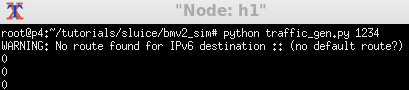
\includegraphics[scale=.6]{figures/arith_ex_1} 
\caption*{H1 sends packet p with result initialized to 0\newline}

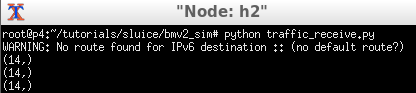
\includegraphics[scale=.6]{figures/arith_ex_2}
\caption*{H2 Receives p with a result header of 14}
\end{minipage}
\end{figure}

All statements in Sluice map to P4 tables and actions. For instance, for the unconditional statement in line 19 of the simple arithmetic example, several P4 actions are generated: one to read \texttt{reg2} into metadata, one to read \texttt{reg1} at index \texttt{a} into metadata, and one to add \texttt{reg1} and \texttt{reg2} metadata and store the result in the transient var \texttt{b}. These actions are shown in \irref{Listing}{ln19}.   

\begin{lstlisting}[caption={P4 Actions for Line 19 of simple\_arithmetic snippet}\label{ln19}, frame=tlrb, basicstyle=\linespread{1.3}\scriptsize]
action action13 () {
    register_read(mdata.reg1, reg1, mdata.a);
}
action action14 () {
    register_read(mdata.reg2, reg2, 0);
}
action action15 () {
    add(mdata.b, mdata.reg1, mdata.reg2);
}
\end{lstlisting}

Conditional statement handling is slightly more complicated. Sluice programs containing if-else blocks undergo a \textbf{branch removal} step akin to a similar transformation used in the Domino compiler~\cite{domino}. Here, any statements inside an if-else block are converted into ternary conditionals. 

\begin{lstlisting}[caption={simple\_arithmetic snippet}\label{brn} after branch removal, numbers=left, firstnumber=1, frame=tlrb, basicstyle=\linespread{1.3}\scriptsize]
import device psa;

packet p: udp(srcPort:1234) {
  result : bit<32>;
}

@ bmv2 : s1, s2, ;
snippet simple_arithmetic() {
    transient a : bit<32> = 2;
    transient b : bit<32> = 6;
    transient c : bit<1>;
    persistent reg1 : bit<32>[3] = {4, 1, 8, };
    persistent reg2 : bit<32> = 1;
    transient if_block_tmp_1 : bit<1>;
    transient tmp_0_if_1 : bit<32>;
    if_block_tmp_1 = a > reg2;
    tmp_0_if_1 = reg2 + b;
    reg1[a] = if_block_tmp_1 ? tmp_0_if_1 : reg1[a];
    reg2 = if_block_tmp_1 ? 7 : reg2;
    c = a > reg2;
    b = reg1[a] + reg2;
    p.result = c ? reg2 : b;
}
\end{lstlisting}

In \irref{Listing}{nobrn} line 15 of the \texttt{simple\_arithmetic} snippet, the assignment of \texttt{reg1[a]} to RHS \texttt{reg2 + b} is conditional on \texttt{a} being greater than \texttt{reg2}. \irref{Listing}{brn} shows this same snippet with branches removed. To remove branches this, a new transient condition variable \texttt{if\_block\_tmp\_1} is generated. It is then set to the single bit result of the original \texttt{if} statement comparison \texttt{a > reg2}. Another transient variable \texttt{tmp\_0\_if\_1} is used to store the value of the RHS, which is used only when the \texttt{if} condition is satisfied i.e. when \texttt{if\_block\_tmp\_1 = 1}. The final conditional assignment to \texttt{reg1[a]} is expressed as a ternary conditional on line 18. If \texttt{if\_block\_tmp\_1 = 1}, \texttt{reg1[a]} is assigned to the RHS, otherwise it is assigned to itself i.e. left alone. A similar ternary assignment based on the condition variable \texttt{if\_block\_tmp\_1} is also created for \texttt{reg2} on line 19. 

Branch removal leads to a sequence of ternary assignments which are in turn converted into P4 match-action tables by the Sluice compiler. Regular assignment statements are converted into a table with a single default action corresponding to the assignment. However, ternary conditional assignments are converted into a table with a match on the binary condition bit and the two corresponding actions. The first action represents assignment to the first ternary operand (in case the condition bit is true or 1,) while the second represents assignment to the second ternary operand (in case the condition bit is false or 0). Sluice populates the control plane with these table entries before packets start flowing through the network. The value of the condition bit is computed in the P4 ingress control block. \irref{Figure}{condP4} displays the compiler-generated P4 tables, actions, ingress control, and control plane entries corresponding to the Sluice code in lines 16-18 of \irref{Listing}{brn}. Note that the condition bit is only set to 1 (via table2, action2) if \texttt{mdata.a > mdata.reg2} in the ingress control block. 

\begin{figure}
\caption{P4 Translation for Sluice Conditional Statement}\label{condP4}
\captionsetup{justification=centering, font=footnotesize,labelfont=footnotesize}
\begin{minipage}{.46\textwidth} 
\begin{lstlisting}[title=P4 Match Action Tables, frame=tlrb, basicstyle=\linespread{1.3}\scriptsize]
table table2 {
    actions {
        action2;
    }
}
table table3 {
    actions {
        action3;
    }
}
table table4 {
    actions {
        action4;
    }
}
table table5 {
    actions {
        action5;
    }
}
table table6 {
    reads {
        mdata.if_block_tmp_1 : exact;
    }
    actions {
        action6;
        action7;
    }
}
\end{lstlisting}
\end{minipage}
\qquad
\begin{minipage}{0.515\textwidth} 
\begin{lstlisting}[title=P4 Actions, frame=tlrb, basicstyle=\linespread{1.3}\scriptsize]
action action2 () {
    modify_field(mdata.if_block_tmp_1, 1); 
}
action action3 () {
    modify_field(mdata.if_block_tmp_1, 0); 
}
action action4 () {
  register_read(mdata.reg2, reg2, 0);
}
action action5 () {
  add(mdata.tmp_0_if_1,mdata.reg2,mdata.b);
}
action action6 () {
  register_write(reg1,mdata.a,mdata.tmp_0_if_1);
}
action action7 () {
}
\end{lstlisting}
\begin{lstlisting}[title=P4 Ingress Control, frame=tlrb, basicstyle=\linespread{1.3}\scriptsize]
if (mdata.a > mdata.reg2) {
    apply(table2);
} else {
    apply(table3);
}
\end{lstlisting}
\begin{lstlisting}[title=Control Plane Entries, frame=tlrb, basicstyle=\linespread{1.3}\scriptsize]
table_set_default table4 action4
table_set_default table5 action5
table_add table6 action6 1 => 
table_add table6 action7 0 => 
\end{lstlisting}
\end{minipage}
\end{figure}

While branch removal does not improve nor significantly degrade performance, it transforms a snippet into straight-line code, greatly simplifying dependency analysis. This analysis is detailed more in next section. 

\newpage
\subsection{Dependency DAG}
The Sluice model allows the possibility for statements to be moved between snippets i.e. between devices. However code movement is inherently dangerous as the semantics of the new program must be the same as those intended by the operator in the original snippet. Consider a simple unconditional assignment statement in snippet A that is moved to snippet B. If the lvalue variable is read again in snippet A (read after write RAW), movement of the statement onto snippet B may change future values of certain variables in snippet A.  To keep track of these variable dependencies within a snippet, a snippet is decomposed into \texttt{atoms} and a directed acyclic graph (DAG) is constructed from these atoms (nodes in the DAG). An atom is a line or the smallest unit of a code in Sluice that needs to be translated to P4. An atom could be a variable declaration, conditional statement, or unconditional statement. A dependency between individual atoms could be RAW, write after write (WAW), or write after read (WAR). This DAG construction is necessary to maintain consistency when performing translation/movement, and to map the stages in switch-pipeline accordingly \footnote{Pipeline stage mapping is relevant for the Tofino architecture, which is not currently supported.}. After the branch removal step, Sluice builds the DAG by maintaining the next and previous atoms for each atom in the snippet. 

The dependency graph for \irref{Listing}{brn} is shown in \irref{Figure}{dag}. The top layer of nodes represents the snippet variable declarations. Arrows represent dependencies between variables in the parent and child nodes. For example, we can trace the use of transient variable \texttt{a} in statements of the snippet. The dependency path for \texttt{a} touches the following nodes in order: \texttt{transient a} $\longrightarrow$ \texttt{if\_block\_tmp\_1 = a > reg2} $\longrightarrow$ \\ \texttt{reg1[a] = if\_block\_tmp\_1 ? tmp\_0\_if\_1 : reg1[a]} $\longrightarrow$ \texttt{c = a > reg2} $\longrightarrow$ \\ \texttt{b = reg1[a] + reg2}.

\begin{figure}
\centering
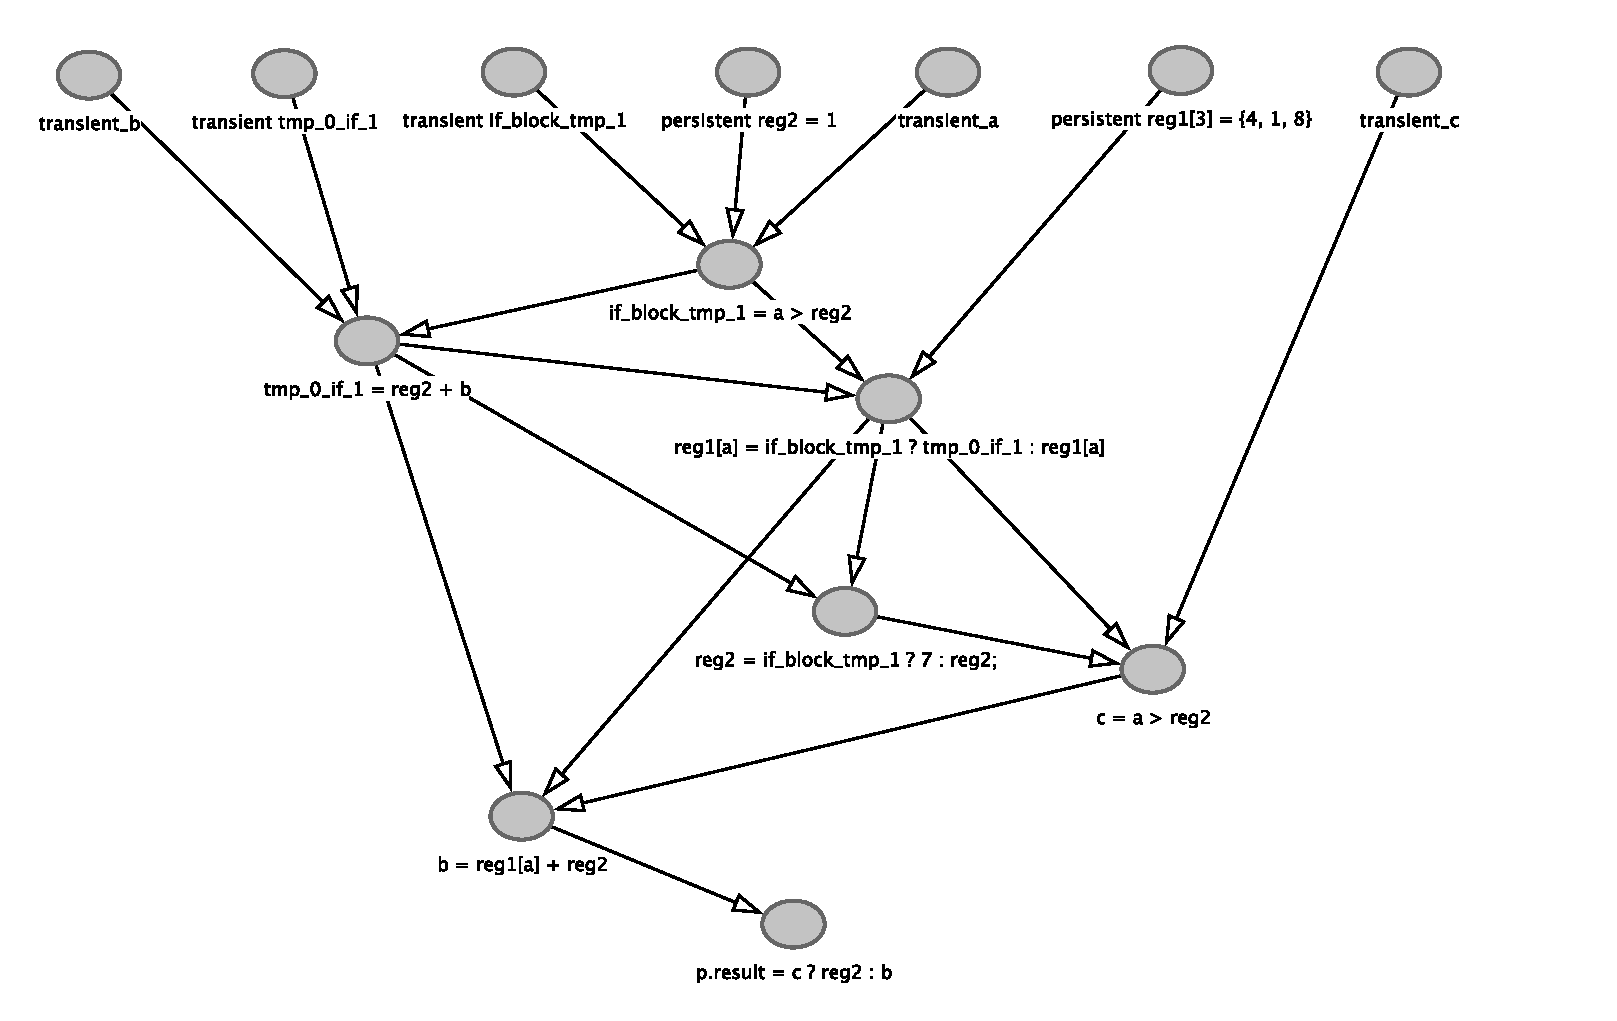
\includegraphics[width=175mm,scale=1]{figures/dependency_dag.pdf}
\caption{Dependency DAG for \irref{Listing}{brn} }\label{dag}
\end{figure}

 

\newpage
\section{Demonstrations} 
In this section, we demonstrate Sluice's functionality and ease of use via two examples: traffic matrix generation for network analysis and a streaming join-filter operation. Videos for these two demos can be found at \cite{traf} and \cite{stream} respectively. Before we describe them further, we provide a description of the Sluice simulator.

\subsection{Sluice Simulator}
The Sluice simulator is written in python and automates much of the aspects of network-wide programming. The operator need only provide a Sluice program and a topology json file outlining the layout of switches and hosts in the network topology. Given the topology file, the simulator generates arp requests for link layer addressing between hosts, determines the shortest routing paths between hosts, and installs forwarding rules on each switch. It uses annotations in the Sluice program to create independent P4 programs for each snippet and run them on their respective devices. In the case that the operator intends to run multiple snippets on a single switch, these snippets will have to be merged to generate a single P4 program. While snippet merging is not currently supported, this is a desired feature and is discussed in the future work section. 

Persistent switch state in registers can be read/written to using the simulator. We provide an API that accesses registers from the control plane using an RPC call over the Apache thrift port corresponding to the switch. For instance, the API function call \texttt{register\_read reg1} returns a list of all values in the array reg1. The simulator also automates the installing of control plane table entries for register initial values and statements in snippets.
\subsection{Traffic Matrix}

\begin{figure}
\centering
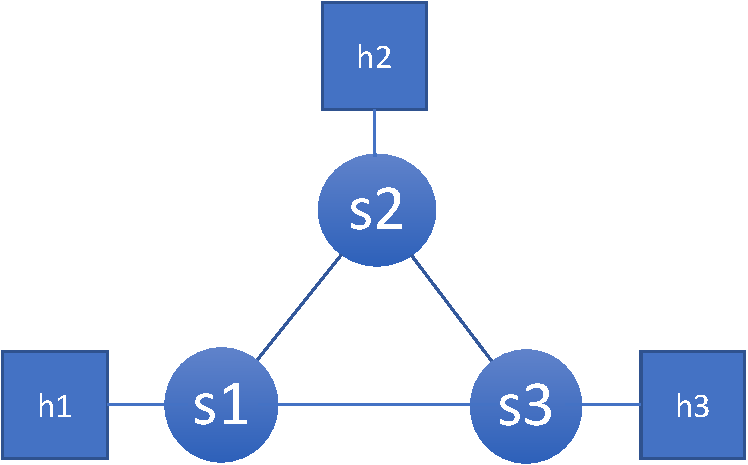
\includegraphics[width=70mm,scale=0.7]{figures/traf_mat_topo}
\caption{Topology For Traffic Matrix Demo}
\end{figure}


Figure 2 displays the Mininet network topology for our traffic matrix demo.
Packets are sent over UDP from each host to all other hosts according to a
Poisson traffic model with mean inter-arrival time of 0.5 seconds. \irref{Listing}{slTraf} is our Sluice program with a single snippet \texttt{traffic\_example}
that is launched on all switches of the network. To run the simulation, the
user passes the Sluice program and network topology to the compiler. The
compiler generates P4 code to run on each switch as well as control plane table
entries for routing packets through the topology.  

\begin{lstlisting}[caption={Sluice Traffic\_Example}\label{slTraf}, frame=tlrb, basicstyle=\linespread{1.3}\scriptsize]
import device psa;

packet p: udp(srcPort:1234)
  nhops : bit<32>;

@ bmv2 : ;
snippet traffic_example()
  persistent cnt : bit<32>[10];
  cnt[psa.ingress_port] = cnt[psa.ingress_port] + 1;
  p.nhops = p.nhops + 1;
\end{lstlisting}
\irref{Listing}{p4Traf} shows the corresponding P4 actions generated by the Sluice compiler to execute the statements in snippet \texttt{traffic\_example}.
\begin{lstlisting}[caption={P4 Actions For Traffic\_Example}\label{p4Traf}, frame=tlrb, basicstyle=\linespread{1.3}\scriptsize]{Name}
action action1 () {
    register_read(mdata.cnt, cnt, standard_metadata.ingress_port);
}
action action2 () {
    add(mdata.cnt, mdata.cnt, 1);
    register_write(cnt, standard_metadata.ingress_port, mdata.cnt);
}
action action3 () {
    add(p.nhops, p.nhops, 1);
}
\end{lstlisting}

\begin{figure}
\centering
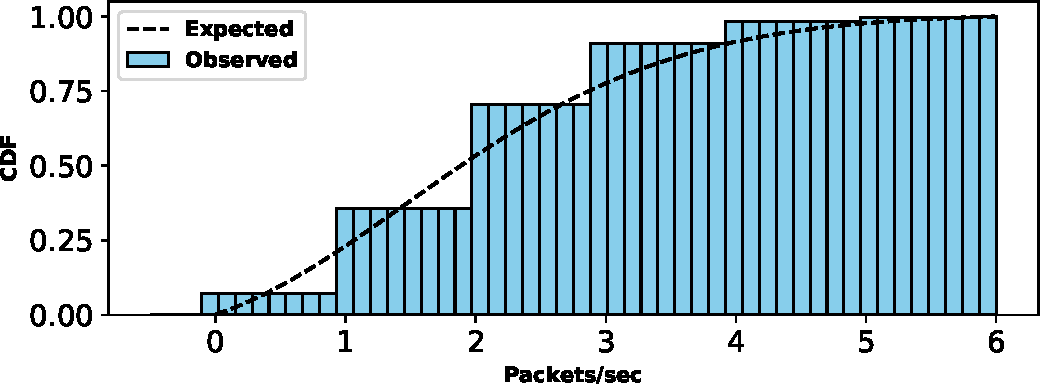
\includegraphics[width=160mm,scale=0.7]{figures/exp_obs_cdf}
\caption{CDF of Packet Rate on link s1-s3}\label{cdf}
\end{figure}

This demo shows how a simple Sluice program can be used to enable each switch
to measure link usage for a specific flow of user-defined packets on UDP
srcPort 1234. Each packet \texttt{p} contains a custom header \texttt{nhops}
that is incremented each time the packet enters a switch to inform the
receiving host of the number of hops the packet took. Each switch maintains a
stateful register counter \texttt{cnt}, indexed by switch ingress port, that
tracks how many packets have entered through that ingress port. Aggregated over
all switches, these counters represent a matrix measuring each link's
usage in the network at a given time. This matrix (residing on the whole
network) is then queried once every second from the control plane to generate
time-series plots of link-utilization for each link. \irref{Figure}{cdf} displays the cumulative
histogram of packet rates on link s1-s3 after collecting data for 15 minutes.
The expected CDF of packet rates \texttt{Poisson}($\mu = 2$
packets/sec) is also plotted to confirm the accuracy of the Mininet emulation.

\subsection{Stream processing}

\begin{figure}
\centering
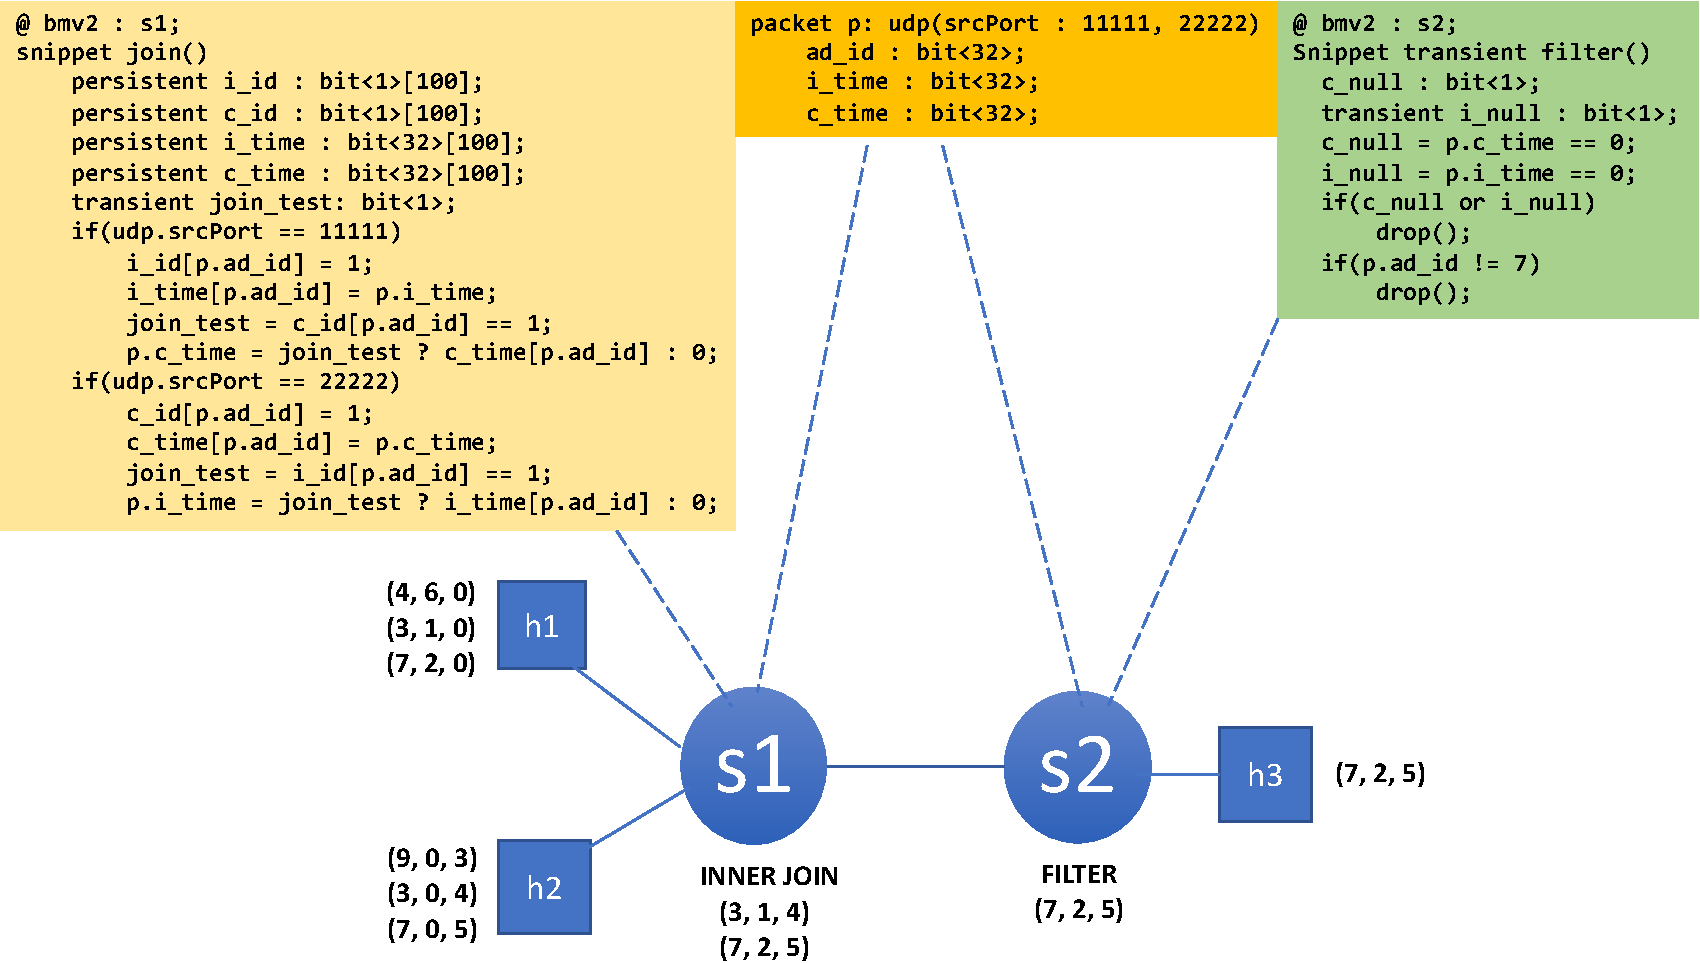
\includegraphics[width=165mm]{figures/streaming_example}
\caption{Streaming example topology, data flow, and code placement on switches}\label{str}
\end{figure}

This example demonstrates a simple join-filter operation between two streams of
tuples. Expressing \texttt{join} in Sluice requires only 31 lines whereas the equivalent P4 code is over 400 lines. 

A stream is an unbounded table where a packet \texttt{p} represents a tuple of
data (\texttt{ad\_id, impression\_time, click\_time}) enclosed in a custom
header. The operator wishes to correlate the two streams to determine the time lag between a user seeing the ad with \texttt{ad\_id = 7} and clicking that same ad. The topology in \irref{Figure}{str} describes the data flow and shows how an
operator query runs on the switches of the network. Host 1 sends a stream of ad
impressions with \texttt{udp.srcPort = 11111} while Host 2 sends a stream of ad clicks with \texttt{udp.srcPort = 22222} . The two streams are
joined on the \texttt{ad\_id} field at s1 (which runs snippet \texttt{join}) and filtered at s2 (which runs snippet \texttt{filter}) when \texttt{ad\_id = 7}. The final result is sent to h3. The MySQL query corresponding to this example is shown below.

\begin{lstlisting}[frame=tlrb, language = SQL, basicstyle=\linespread{1.3}\scriptsize]{Name}
SELECT adId, impression_time, click_time 
FROM impressions i 
INNER JOIN clicks c ON i.adId = c.adId
WHERE i.adId = 7
\end{lstlisting}

Traditional join algorithms such as nested loop join, sort-merge join and hash join all require loops. On the other hand, Sluice is able to accomplish joins using loop-free semantics under several assumptions. Let us assume that the impression packet (3, 1, 0) arrives first at \texttt{s1}. The \texttt{ad\_id} field with value 3 is used as an index into the \texttt{i\_id} register and this register is set to 1 at the index 3. The \texttt{ad\_id} field is also used as an index into the \texttt{i\_time} register, which is updated at index 3 with the impression time of 1. In this way, the \texttt{i\_id} register serves as a bit vector indicating whether or not the switch has seen particular ad impressions whereas the \texttt{i\_time} register stores the impression times for the ad impression tuples the switch has seen so far. 

Let us now assume that the click packet (3, 0, 4) arrives at \texttt{s1}. As in the case of impression packets, a pair of registers, \texttt{c\_id} and \texttt{c\_time}, are maintained to record arriving ad click packets. At this point, we check whether the switch has already seen an impression with an \texttt{ad\_id} equal to that of the current click packet i.e. 3. If the value of bit \texttt{i\_id[p.ad\_id]} is 1, the impression has been seen and the corresponding impression time \texttt{i\_time[p.ad\_id]} is written to the packet header \texttt{p.i\_time}. Since the impression packet (3, 1, 0) was already seen, the value of \texttt{i\_id[3]} is indeed 1 and the impression time \texttt{i\_time[3] = 1} is written to the click packet to yield (3, 1, 4). 

The result of \texttt{s1}, (3, 1, 4), now flows to \texttt{s2} where it is filtered on \texttt{ad\_id = 7}. Since the ad\_id 3 is not equal to 7, the packet is simply dropped. Although not shown here, a similar analysis can be done when a click arrives before a matching impression.  

It is important to note several caveats to this algorithm. For instance, if there are multiple impressions for the same ad, only a single tuple will be stored on the switch at any time since the primary key ad\_id is duplicated and the corresponding index gets overwritten. This is equivalent to an unresolved hash collision. In this case, it is simple to resolve by tracking impressions with an extra key, for example, an impression\_id that is unique among impressions of a particular ad. 

Another caveat is that the maximum number of unique tuples that can be stored for joining is limited by the total TCAM and SRAM memory of the target hardware. While a capacity of 100 unique ad\_ids is suitable for this demo, whether it is suitable for a different application depends on how fast the streams are being sent. For example, suppose the switch only supports 30Mb of total memory and all 30Mb are used for storing tuples. If impressions arrive at a rate of 30Mb/s and clicks arrive at a slower rate of 10Mb/s, then switch memory will be exhausted in 1 second with a majority of register entries storing tuples for impressions as opposed to clicks. Due to varying send rates, a large time lag ensues between possible impression/click join matches. In addition, since switch memory is quickly exhausted, many tuples are overwritten causing possible matches to not be recognized. Thus the operator may have to fine-tune sending rates to ensure that the probability of failed matches is minimized.    

\newpage
\section{Future Work}
\subsection{An optimizing Sluice compiler.} We envision using the dependency DAG to
provide several automatic optimizations or code transformations. For example,
it is possible that certain lines of code in a snippet cannot be run on the
device annotated by the operator, e.g., programmable switching chips have
limited support for floating point or complex string operations. Code
containing such features must be moved to the control plane or an end host data
plane while at the same time, preserving the original program semantics
intended by the operator. Doing this automatically would free the Sluice
programmer from reasoning about these semantics. Consider a case where a switch needs to carry out some computations based on packet headers alone without reading or writing switch-resident state. One example is taking the product of two headers and writing it into a third header without involving any switch state in the process. This pattern occurs in the congestion-control protocol XCP~\cite{xcp}, which needs to compute the product of the current RTT and the packet size and divide it by the current congestion window. All three of these variables are present in the packet and need not be computed on the switch. This makes it simpler to offload the computation to an end host where precise floating point division and multiplication are much easier to carry out~\cite{sharma}

In certain situations, code movement cannot be performed even when floating point accuracy is desired. Consider the snippet in \irref{Listing}{ewma} which computes an exponentially weighted moving average (EWMA with $\alpha=0.2$) of queuing latencies and writes the EWMA to a packet header \texttt{result}. 

\begin{lstlisting}[caption={EWMA}\label{ewma}, frame=tlrb, basicstyle=\linespread{1.3}\scriptsize]
import device psa;

packet p: udp(srcPort:1234)
  result : bit<32>;

@ bmv2 : ;
snippet ewma() {
    persistent avg : bit<32>;
    transient latency : bit<32>;
    avg = 8 * avg;
    avg = avg / 10;
    latency = psa.timestamp_egress - psa.timestamp_ingress;
    latency = 2 * latency;
    latency = latency / 10;
    avg = avg + latency;
    p.result = avg;
\end{lstlisting}

The statements computing EWMA include division and multiplication and must accurate to several decimal places. The EWMA itself exists as a persistent variable \texttt{avg} on the switch which is updated with every packet \texttt{p} on the flow \texttt{udp.srcPort=1234}. In addition, it is written to the \texttt{result} header of each packet \texttt{p}. To match these stateful semantics, all statements must be run on the switch and cannot be moved onto the control plane or an end-host. The result must also be approximated with fixed point arithmetic since floating point is not supported in switch hardware. 

Fortunately, it is straightforward to represent a multiplication using bit shifts and adds by writing out both numbers in binary. For instance, say we were multiplying 27 by 5. As shown below, this can be implemented by first shifting 27 left by 2 bits and then adding 27.\\
$27 * 5 (1)$\\
$= (11011) * (101)$\\
$= (11011) * (1 * 2^2 + 0 * 2^1 + 1 * 2^0)$\\
$= (11011) << 2 + (11011) << 0$\\
$= (11011) << 2 + (11011)$\\
Similarly, we can approximate division by treating it as multiplication by the inverse and using right shifts instead of left shifts. Assuming a budget on N number of shifts (and hence N - 1 adds), we can use a lookup table to compute the shift coefficients for each value of the smaller of the two operands. For instance, in the example above where we multiply 27 by 5, this lookup table will tells us that to multiply by 5, we need to use the shift values 2 and 0 if we have a budget of two shifts and the shift value 2 alone if we have a budget of one shift.
The more the budget on the number of shifts, the closer we can approximate the original multiplication or division. However, the smaller the budget on the number of shifts, the more we can compress the lookup table. For instance, if we are permitted only one shift, then the lookup table returns the nearest exponent of 2 for each value of the smaller operand, allowing us to significantly compress the lookup table. As one example of compression, assuming 8-bit operands, the shift value for all operands from 17 to 31 will be 4 and can be represented by a single TCAM entry mapping the bit pattern 0001**** to the shift value 4.

\subsection{Supporting multi-tenancy.} Another area of future work is allowing
Sluice to support multiple tenants with their own Sluice
programs running on their own virtual networks overlayed on the same physical
topology. If each tenant wants to run their own network-wide program on their
virtual topology, the network operator will need to merge all these into one
data plane implementation that runs on the entire physical network. Extending
Sluice to support this multi-tenancy use case would allow us to provide the
same benefits to the data plane that multi-tenant network
virtualization~\cite{multitenant} provided for the control plane.



\newpage
\section{Appendix}
\subsection{Sluice grammar} 
\begin{lstlisting}[basicstyle=\linespread{1.3}\scriptsize,  numberstyle=\tiny, backgroundcolor = \color{teagreen}, frame=tlrb]
program:
	imports packets snippets				
	| packets snippets
	;
imports:
	imports import
	| import
	;
import:
	"import device" IMPORT_ID
	;
packets:
	packets packet
	| packet
	;
packet:
	"packet" PACKET_ID packet_base packet_parser_condition packet_fields
	;
packet_base:
	"tcp" | "udp" | "ipv4" | "ethernet"
	;
packet_fields:
	packet_fields packet_field
	| packet_field
	;
packet_field:
	IDENTIFIER var_type type_qualifier
	;
packet_parser_condition:
	IDENTIFIER value
	| Empty
	;
snippets:
	snippets snippet
	| snippet
	;
snippet:
	device_annotation "snippet" SNIPPET_ID variable_decls ifblocks
	;
device_annotation:
	"@" DEVICE_TYPE device_vector
	;
device_vector:
	device_vector "," IDENTIFIER
	| IDENTIFIER
	;
variable_decls:
	variable_decls variable_decl
	| variable_decl
	;
variable_decl:
	IDENTIFIER initial_values var_type
	;
initial_values:
	initial_values "," initial_value
	| initial_value
	;
initial_value: 
	value
	;
var_type:
	var_info type_qualifier
	;
var_info:
	bit_array | packet
	;
bit_array:
	bit_width var_size
	;
bit_width: 
	digits
	;
var_size: 
	digits
	;
type_qualifier:
	"Persistent" | "Transient" | "Field"
	;
value: 
	digits
	;
digits: 
	digit+
	;
digit:  
	0 | 1 | 2 | 3 | 4 | 5 | 6 | 7 | 8 | 9
	;
ifblocks:
	ifblocks ifblock
	| ifblock
	;
ifblock:
	id condtype condition statements
	;
id: 
	digits
	;
condtype: 
	1 | 2 | 3
	;
condition:
	expr
	; 
statements:
	statements statement
	| statement
	;
statement:
	lvalue "=" expr
	;
expr:
	operand expr_right
	;
operand:
	lvalue | value
	;
lvalue:
	scalar | array | field
	;
scalar:
	IDENTIFIER
	;
array:
	IDENTIFIER "[" operand "]"
	;
field:
	IDENTIFIER "." IDENTIFIER
	;
expr_right:
	BinOp | Cond | Empty
	;
BinOp:
	"and" | "or" | "+" | "-" | ">>" | "<<" | "==" | "!=" | "<" | ">" | ">=" | "<="
	;
Cond:
	operand "?" operand
	;
\end{lstlisting}

\subsection{Sluice Compiler Source Code} 

The Sluice compiler is written in rust while its simulator is written in python and bash. Source code can be found at \cite{sluiceSrc}. The lines-of-source breakdown is shown below.

\begin{center}
 \begin{tabular} {|c c c c c|} 
 \hline
 Language &  files & blank & comment & code  \\ [0.5ex] 
  \hline\hline
Rust &	15  & 689 & 419 &  4836\\
 \hline\hline
P4&	58 & 110 & 0 & 603 \\
 \hline
Python& 6 & 153 & 176 & 528 \\
 \hline
JSON&	62 & 0 & 0 & 62 \\
 \hline
Bourne Shell&	5 & 29 & 15 & 55 \\
 \hline
make & 1 & 15 & 2 & 31 \\
 \hline
Markdown & 3 & 5 & 0 & 18 \\
 \hline
TOML & 1 & 1 & 0 & 9 \\
 \hline
 \textbf{SUM} & \textbf{151} & \textbf{1002} & \textbf{612} & \textbf{6142} \\
 \hline
\end{tabular}
\end{center}


\newpage
\bibliographystyle{unsrt}
\bibliography{thesis.bib}


\end{document}



